\documentclass{article}
\usepackage{amsmath}
\usepackage{tikz}

\begin{document}

\section*{Problemas de modelado II: asignación}

6. En el pueblo de Asignasonia las fiestas de casamiento son muy peculiares y extrañamente frecuentes. Las invitaciones a la fiesta nunca son personales sino familiares: cada persona invitada asiste siempre con todos sus familiares solteros, a quienes se les reservan mesas especiales de solteros. Además, hay una regla no escrita que establece un límite \( c_{ij} \) a la cantidad de solteros de la familia \( i \) que pueden sentarse en la mesa \( j \). Esta forma de festejar es la que, aparentemente, aumenta la cantidad de casamientos futuros. Desafortunadamente, el esfuerzo que implica mantener viva esta tradición está llevando a que varias parejas eviten el compromiso marital. Es por esto que la intendencia de Asignasonia requiere un algoritmo que resuelva el problema de asignación de los solteros a sus mesas.

\begin{enumerate}
    \item[a)] Proponer un modelo de flujo que, dados los conjuntos \( F = \{f_1, \ldots, f_{|F|}\} \), \( M = \{m_1, \ldots, m_{|M|}\} \) y \( C = \{c_{ij} \mid 1 \leq i \leq |F|, 1 \leq j \leq |M|\} \), determine una asignación que respete las tradiciones sabiendo que:
    \begin{itemize}
        \item La familia \( i \) está formada por \( f_i \) personas solteras.
        \item La mesa \( j \) tiene \( m_j \) lugares disponibles para solteros.
        \item En la mesa \( j \) solo pueden sentarse \( c_{ij} \) solteros de la familia \( i \).
    \end{itemize}
    
    \item[b)] Dar una interpretación a cada unidad de flujo y cada restricción de capacidad.
    
    \item[c)] Determinar la complejidad de resolver el modelo resultante con el algoritmo de Edmonds y Karp.
\end{enumerate}

Definimos una red de flujo, con fuente \( s \) y sumidero \( t \). Conectamos a todos los familiares \( f_i \) con todas las mesas \( m_j \) con capacidad \( c_{ij} \). Conectamos la fuente \( s \) con todas las familias con capacidad \( f_i \) respectivamente. Luego conectamos todas las mesas al sumidero \( t \) con capacidad \( m_j \) respectivamente.


\begin{figure}[h]

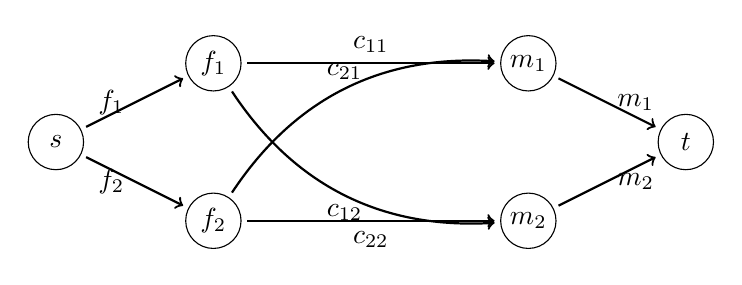
\begin{tikzpicture}[
    vertex/.style={circle, draw, minimum size=20pt, inner sep=0pt},
    edge/.style={->, thick, shorten >=2pt, shorten <=2pt}
  ]
  % Vertices representing families and tables
  \node[vertex] (f1) at (0,2) {$f_1$};
  \node[vertex] (f2) at (0,0) {$f_2$};
  \node[vertex] (m1) at (4,2) {$m_1$};
  \node[vertex] (m2) at (4,0) {$m_2$};
  
  % Edges with capacities
  \draw[edge] (f1) to node[above] {$c_{11}$} (m1);
  \draw[edge] (f1) to[bend right] node[below] {$c_{12}$} (m2);
  \draw[edge] (f2) to[bend left] node[above] {$c_{21}$} (m1);
  \draw[edge] (f2) to node[below] {$c_{22}$} (m2);
  
  % Source and sink
  \node[vertex] (source) at (-2,1) {$s$};
  \node[vertex] (sink) at (6,1) {$t$};
  
  % Connections from source to families
  \draw[edge] (source) to node[left] {$f_1$} (f1);
  \draw[edge] (source) to node[left] {$f_2$} (f2);
  
  % Connections from tables to sink
  \draw[edge] (m1) to node[right] {$m_1$} (sink);
  \draw[edge] (m2) to node[right] {$m_2$} (sink);
\end{tikzpicture}
\caption{Modelo de Red con 2 familias y 2 mesas}
\end{figure}



Dado un flujo máximo, el flujo entrante a cada mesa representa la cantidad de personas que se van a sentar ahí. En particular, viendo de donde vienen podemos saber de qué familia es. Para que todos se puedan sentar debería ocurrir que las aristas que van de la fuente a las familias deben estar saturadas.

Complejidad Edmonds-Karp: \( O(nm^2) \).


Hay \( \Theta (\binom{|F| + |M|}{2} + |F| + |M|) =  \Theta(F^{2} + FM + M² ) \) aristas.

Vertices: \( \Theta ( |F| + |M| + 2 ) \).

Entonces, la complejidad final es de \( O((|F| + |M| + 2) \cdot (F^{2} + FM + M² )^2) \).

\end{document}
